\documentclass{article}

\usepackage{annalhq}

\usepackage[utf8]{inputenc}
\usepackage[T1]{fontenc}
\usepackage{hyperref}
\usepackage{url}           
\usepackage{booktabs}
\usepackage{tabularx}
\usepackage{amsfonts}
\usepackage{nicefrac}
\usepackage{microtype}     
\usepackage{cleveref}    
\usepackage{lipsum}
\usepackage{graphicx}
\usepackage{natbib}
\usepackage{doi}
\usepackage{subcaption}

\title{\emph{OREACLE}: A novel framework for rockfall prediction}

%\date{Sept 27, 2025}
% 
%\date{}

\newif\ifuniqueAffiliation

\uniqueAffiliationtrue

\ifuniqueAffiliation
\author{Annalhq Shaikh\\
	Department of CSE AIML\\
	RCOEM\\
	Nagpur, 440001 \\
	\texttt{shaikhah@rknec.edu} \\
	%% more athors
	% \And
	% Annalhq H.~Shaikh \\
	% Department of CSE AIML\\
	% RCOEM\\
	% Nagpur, 440001 \\
	% \texttt{shaikhah@rknec.edu} \\
}
\else

\fi

% Uncomment to override  the `A preprint' in the header
\renewcommand{\headeright}{} %add text over here! lol
\renewcommand{\undertitle}{}
\renewcommand{\shorttitle}{\textit{Oreacle: Technical approach}  }

%%% Add PDF metadata 
%%% check the metadata with $ pdfinfo template.pdf

\hypersetup{
pdftitle={OREACLE: A novel framework for rockfall prediction},
pdfsubject={oreacle architecture},
pdfauthor={Annalhq H.~Shaikh},
pdfkeywords={PointNet++, GRU, LSTM, Topographic analysis},
% my link setup
colorlinks=true,
linkcolor=blue,    % internal links (\ref, \cite)
filecolor=blue,    % file links
urlcolor=blue,     % external URLs ( \url, \href)
citecolor=blue,    % citation links
}

\begin{document}
\maketitle

\begin{abstract}
We propose the Oreacle, a framework which uses fuses novel techniques to glue together data from UAVs, LiDAR and misc. Sensor data and predicts and forecasts the rockfall in real-time. It is designed to take in real time series data with the respective fallback system in case of sensor malfunctions. 

Traditional monitoring methods often lack the spatial coverage, temporal frequency, and prediction capabilities required to preemptively mitigate these dangers. The proposed architecture is based off four key pillars: (1) High resolution topological geostructural characterization of mine using UAV based LiDAR and advanced 3D deep learning models such as RandLA-Net, KPConv and PointNet++. (2) Real-time analysis of in-situ geotechnical sensor data using efficient and accurate time-series models like Temporal Convolutional Networks (TCNs) (3) A sophisticated multi-modal fusion and ensemble learning strategy to combine spatial and temporal data streams into a single (4) A scalable centralized system for alert dispatching.
\end{abstract}

% keywords can be removed
\keywords{PointNet++ \and GRU \and LSTM \and Topographic Analysis}

\section{Geostructural Characterization via UAV-Based 3D Point Clouds}
The foundational layer of any robust rockfall prediction system is a precise and frequently updated three-dimensional model of the mine's topography. This geostructural characterization serves to identify the static and slowly evolving conditions that create the potential for instability, such as adverse joint orientations, fractures, and gradual deformation. UAVs have emerged as indispensable tools for this task, offering a safe, cost-effective, and rapid means of capturing detailed data over large and inaccessible areas.   

\subsection{Data acquisition strategy: UAV Photogrammetry and LiDAR}
The primary objective of the data acquisition phase is to generate accurate and reproducible Digital Terrain Models (DTMs) and Digital Elevation Model (DEMs) of the mine's highwalls. The choice of sensor technology is a critical first step.   

\begin{figure}[h!]
	\centering
	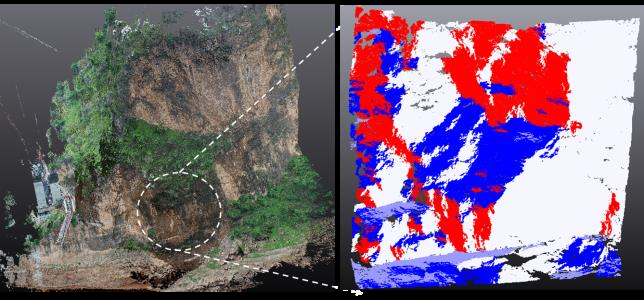
\includegraphics[width=0.7\linewidth]{figures/uav-tls.png}
	\caption{Multi-source 3D point clouds fusion from TLS-UAV technologies,  joint identification results of the representative area and the color band joint sets similar orientations. \cite{3dCloudFusion}}
	\label{fig:fig1}
\end{figure}


\textbf{UAV-LiDAR} offers significant advantages for geotechnical applications. It operates independently of ambient lighting, allowing for consistent data collection in shadowed areas or during various times of day. Crucially, its ability to penetrate vegetation provides a more accurate "bare-earth" model of the rock face, which is essential for identifying underlying geological structures. The high point densities achieved by modern LiDAR systems, often reaching hundreds of points per square meter, are exceptionally well-suited for characterizing the complex geometry of steep and irregular slopes. \cite{land14061193}

\textbf{UAV-Photogrammetry}, which utilizes Structure-from-Motion (\textbf{SfM}) algorithms to generate 3D models from overlapping 2D images, presents a lower-cost alternative. This method is highly effective for creating detailed, textured 3D models and orthophotos that are valuable for visual inspection and the identification of geological features like discontinuities, joint orientations, and fracturing frequency. Advanced SfM processing workflows can detect centimeter-scale changes between surveys, offering a powerful tool for early-warning deformation monitoring.   

For maximum fidelity, a Hybrid Approach that fuses data from UAV-based sensors with Terrestrial Laser Scanning (TLS) can be employed. This strategy enhances both spatial coverage and point cloud density, leading to more comprehensive and detailed slope models that capture features from multiple angles and perspectives \citet{3dCloudFusion}

\section{Point Cloud Processing for Discontinuity and Precursor Identification}
After acquiring a high-density 3D point cloud, it's processed to extract key geotechnical parameters, focusing on the rock mass's discontinuities (joints, faults, bedding planes). Traditional methods analyze parameters like orientation, spacing, and persistence of these features. Using algorithms like RANSAC, planes are fitted to the point cloud, helping identify unstable rock blocks. Unlike image-based methods, this approach can detect failure planes without visible cracks. More advanced methods, such as the ROKA algorithm, perform kinematic stability analysis on 3D point clouds, identifying areas prone to failure types like planar sliding, wedge failure, or toppling. \cite{ROKA}

\subsection{Deep Learning Architectures for 3D Point Cloud Segmentation}
While traditional methods work well, deep learning can learn subtle features linked to instability beyond what predefined geometric rules can capture. For this, we need neural networks that handle unstructured point cloud data directly.

\textbf{PointNet++} is a works efficiently for local high alert zones in open-pits, using hierarchical feature learning to capture local geometric detail. However, its computational load makes it difficult to scale to large open-pit mines with billions of points.

\begin{figure}[h!]
	\centering
	\begin{subfigure}[b]{0.48\linewidth}
		\centering
		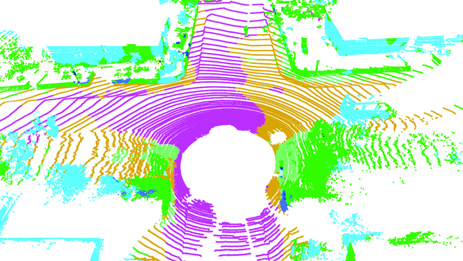
\includegraphics[width=\linewidth]{figures/randla/pointnet.png}
		\caption{PointNet++: \textbf{(2.4s)}}
		\label{fig:PointNet}
	\end{subfigure}
	\hfill
	\begin{subfigure}[b]{0.48\linewidth}
		\centering
		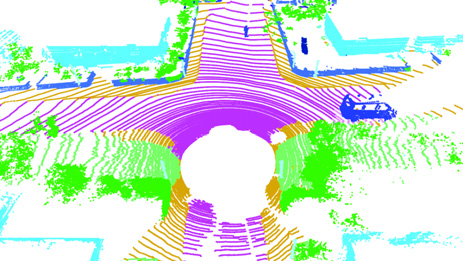
\includegraphics[width=\linewidth]{figures/randla/randla.png}
		\caption{RandLA-Net: \textbf{(0.04s)}}
		\label{fig:modelB}
	\end{subfigure}
	\caption{Time comparison of Semantic segmentation results between PointNet and RandLA-Net \cite{randlanet}}
	\label{fig:cnnComparison}
\end{figure}

\textbf{RandLA-Net} is well-suited for large-scale segmentation tasks. It uses random sampling to reduce point cloud size and a lightweight feature aggregation module to retain important geometric details. Its speed and scalability make it ideal for mine-wide scans, such as identifying rock faces, vegetation, and haul roads. \cite{randlanet}

\textbf{KPConv} introduces deformable kernel point convolutions that adapt to the local geometry of the data. This flexibility makes it particularly effective for capturing the complex, irregular features of rock mass discontinuities—ideal for detailed analysis in high-risk areas.

A tiered strategy works best: use RandLA-Net for broad segmentation and KPConv for fine-grained fracture characterization. While PointNet++ remains important at local scale.


\begin{table}[h!]
	\centering
	\renewcommand{\arraystretch}{1.3}
	\begin{tabularx}{\textwidth}{@{} l X X X X X @{}}
		\toprule
		\textbf{Model} & \textbf{Core Concept} & \textbf{Scalability (Points/Scan)} & \textbf{Computational Cost} & \textbf{Memory} & \textbf{Key Advantage} \\
		\midrule
		\textbf{PointNet++} & Hierarchical feature learning in local neighborhoods & Medium ($10^4$–$10^5$) & High & High & Captures fine-grained local geometry \\
		\textbf{RandLA-Net} & Random sampling with local feature aggregation & Very High ($>10^6$) & Low & Low & Extreme efficiency and speed on massive point clouds \\
		\textbf{KPConv} & Convolution with weights located by learnable kernel points & High ($10^5$–$10^6$) & High & High & Deformable kernels adapt to local geometry \\
		\bottomrule
	\end{tabularx}
\vspace{2pt}
	\caption{Comparison of 3D Point Cloud Processing Models}
\end{table}

\section{Real-Time Analysis of Geotechnical Sensor Time-Series Data}

\begin{figure}[h!]
	\centering
	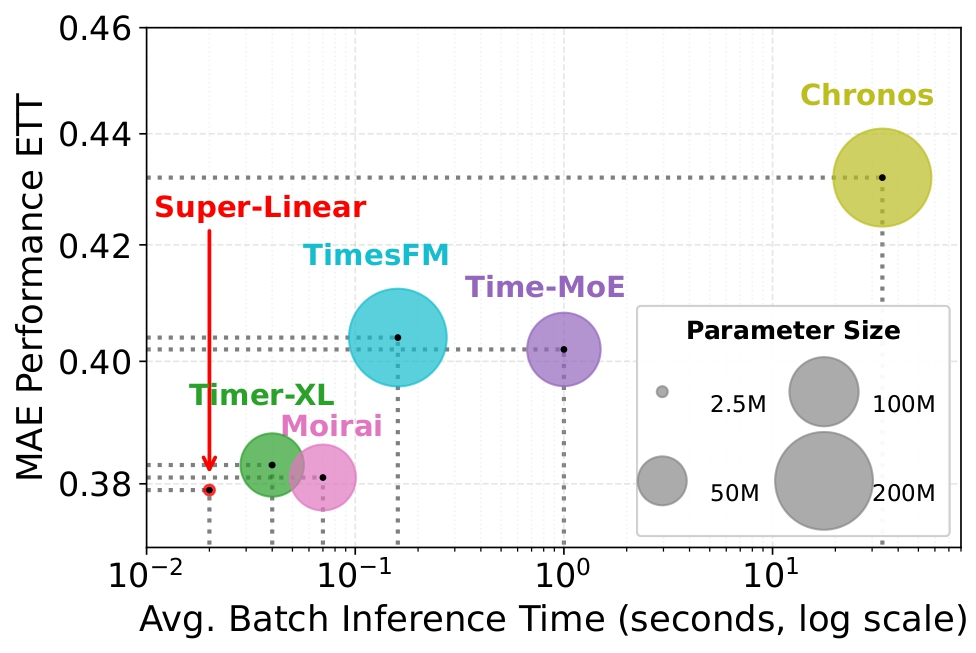
\includegraphics[width=0.7\linewidth]{figures/superlinear.jpg}
	\caption{Performance versus inference time trade-off across different prominent pretrained TSF models. \cite{superlinear}}
	\label{fig:fig1}
\end{figure}

3D point clouds provide detailed spatial data of mine structures but are typically captured intermittently. To monitor real-time dynamic behavior, a network of in-situ geotechnical sensors is needed. These sensors provide continuous time-series data that reveal temporal patterns—such as deformation or changing pore pressures—indicating potential failures.

Sensor Suite and Data Characteristics
A comprehensive monitoring system should include extensometers, inclinometers, piezometers, and microseismic sensors. These instruments can be integrated for real-time data transmission to a central processor.

Geotechnical time-series data is complex, often non-linear and non-stationary. For example, landslide displacement exhibits a long-term trend with periodic fluctuations influenced by factors like rainfall. Analyzing these multi-scale temporal dependencies is a key challenge for modeling.

Recurrent Neural Networks (\textbf{RNNs}) for Temporal Modeling
Long Short-Term Memory (\textbf{LSTM}) networks, a type of RNN, are effective at capturing long-term dependencies in sequential data. Their gating mechanisms help manage the vanishing gradient problem. LSTMs have been applied to landslide prediction by decomposing signals into trend and periodic components.

Gated Recurrent Unit (\textbf{GRU}) networks simplify the LSTM architecture, improving computational efficiency without sacrificing performance. GRUs can outperform LSTMs, especially with smaller datasets.

\textbf{Advanced Alternatives}: Temporal Convolutional Networks (TCNs)
TCNs, which use stacked 1D convolutional layers, offer faster and more efficient processing than RNNs. Their causal and dilated convolutions allow them to capture long-term dependencies while enabling parallel processing, reducing training time. Studies show TCNs often outperform LSTMs and GRUs in forecasting tasks.

\section{Model architecture}
\begin{figure}[h!]
	\centering
	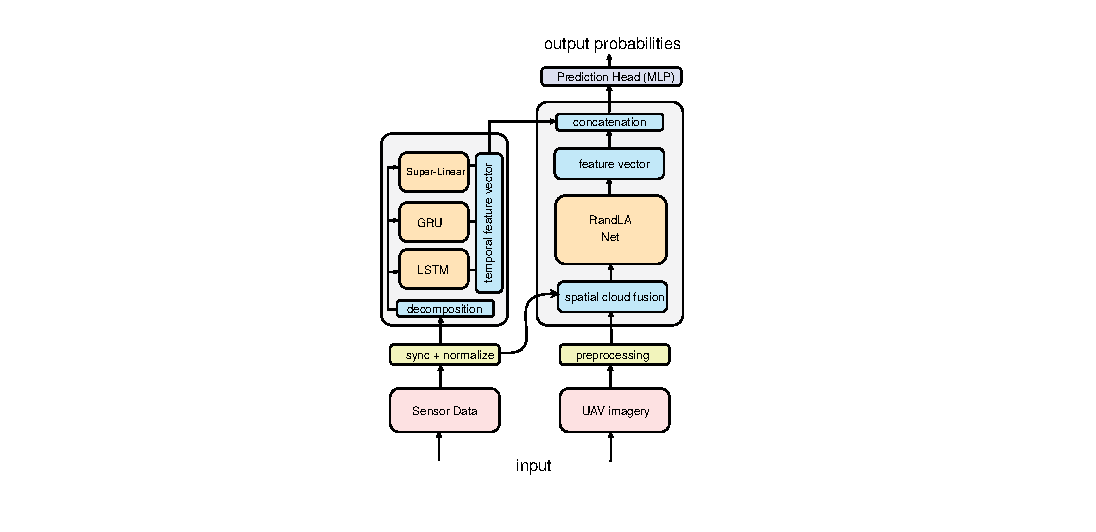
\includegraphics[width=1\linewidth]{figures/architecture.pdf}
	\caption{End-to-end model architecture for Oreacle}
	\label{fig:fig1}
\end{figure}


\section{Dashboard and Alerting System Design}

The final output of the system must be clear, intuitive, and actionable for non-ML experts.

Dashboard Design: The monitoring dashboard should serve as the primary interface for geotechnical engineers. Instead of displaying raw model outputs, it should track and visualize key performance indicators (KPIs) that have direct physical meaning. Drawing from best practices in geotechnical monitoring dashboards, essential KPIs include :   

Displacement Velocity and Acceleration: The rate of change of movement is often more indicative of impending failure than the absolute displacement.

Model Confidence Score: The probabilistic output from the final ensemble model, indicating the system's certainty in its prediction.

Time-to-Threshold Forecast: A projection of when a monitored parameter (e.g., settlement, lateral displacement) is expected to breach a predefined safety limit.

Probability-Weighted Geo-Risk Index: A single, high-level score that aggregates the risks across multiple monitored slopes, allowing management to prioritize attention.

Sensor Data Health: A status overview of all physical sensors to ensure that decisions are being made on complete and timely data.

Real-Time Alerting System: The system must be capable of issuing immediate alerts when the predictive model indicates a high-risk situation. The alerting system should be tiered (e.g., Level 1: Monitor, Level 2: Warning, Level 3: Critical Alarm) and deliver notifications through multiple channels (e.g., mobile app, SMS, desktop notifications) to ensure they reach the appropriate personnel. 1  Alerts must be integrated with the mine's overall emergency response plan and provide clear, concise information, including the location, risk level, and primary contributing factors identified by the model.
\bibliographystyle{unsrtnat}
\bibliography{references} 

\end{document}
